% !TEX root = thesis.tex
\chapter{Approach}
\label{chap:approach}
This chapter describes our approach to predicting the mutation score of a source code unit under test based on source code and test suite metrics data. Our approach at a high-level can be summarized in the following steps:

\begin{enumerate}
	\item Collect mutation score data of the \gls{sut}.
	\item Collect source code metric data of the \gls{sut}.
	\item Collect test suite metrics data of the \gls{sut}.
	\item Synthesis collected data together and store it within a database.
	\item Construct classification model
	\item Predict with classification model
\end{enumerate}

In Section~\ref{sec:approach_process} we describe each step of our process in detail, according to the overview presented in Figure~\ref{fig:process}. Then in Section~\ref{sec:approach_prediction} we describe how we use the produced classification model of our approach for predictions. We mention related works to our research in Section~\ref{sec:approach_related_work}.

\begin{figure}[!tb]
  \centering
  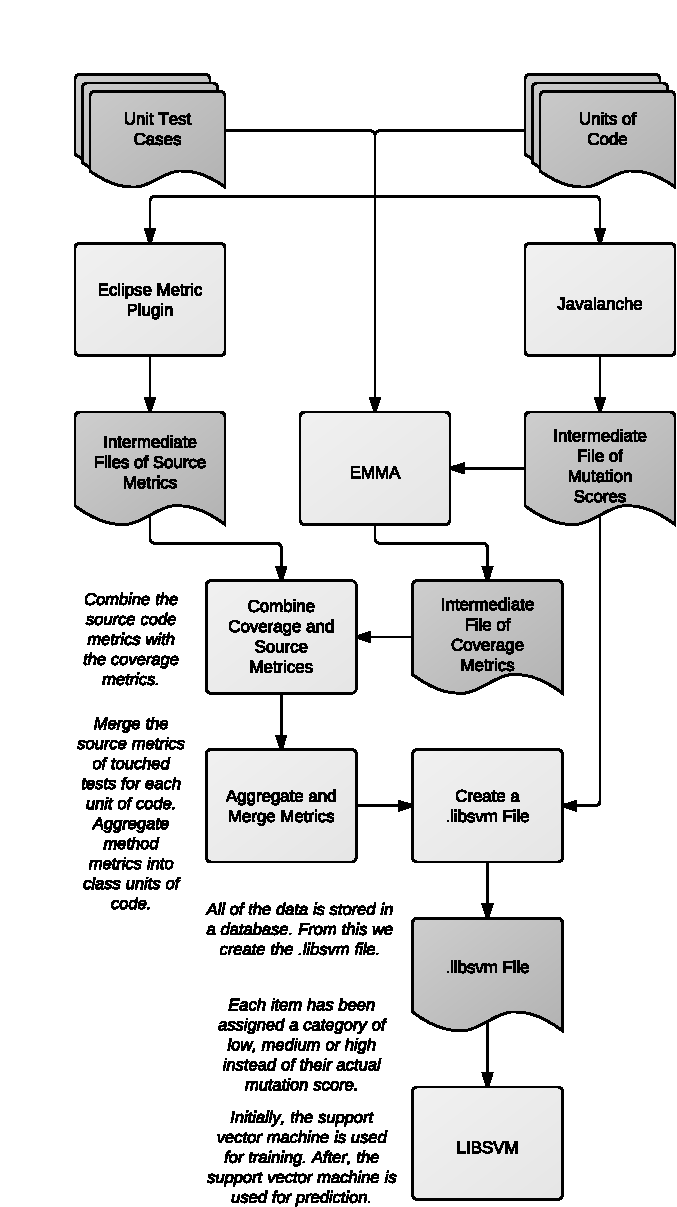
\includegraphics[width=11cm]{figures/process.pdf}
  \caption{Our training process for predicting mutation scores of source code units.}
  \label{fig:process}
  \vspace{2mm}
  \hrule
\end{figure}


\section{Process}
\label{sec:approach_process}
Our process for mutation score prediction using source code and test suite metrics is shown in Figure~\ref{fig:process}. The complete set of source code and test suite metrics used in our process are shown in Table~\ref{tab:metrics}. We grouped our metrics into logical feature sets (see Table~\ref{tab:feature_sets}) so we can manipulate the groupings later in Chapter~\ref{chap:experiment} to understand the benefits of each feature set. Further mention of the feature sets will be referred to by their corresponding set (from Table~\ref{tab:feature_sets} -- \ding{172}, \ding{173}, \ding{174}, \ding{175}), and metrics by their abbreviation (from Table~\ref{tab:metrics} -- NBD, NOF, LCOM, etc\ldots). Supervised machine learning techniques required a model first before any predictions are made (as mentioned in Section~\ref{sec:background_machine_learning}). To achieve this, our process first relies on the notion of acquiring known data to construct the appropriate \gls{svm} model for future prediction. As mentioned in the motivation (see Section~\ref{sec:introduction_motivation}), our approach aims to reduce the amount of mutation testing done in iterative development. If our technique generalizes well, then it can be possible to build a comprehensive model and predict on different software systems without any prior mutation testing. This will be explored in Chapter~\ref{chap:experiment}.

\begin{table}[!tb]
  \centering
  \rowcolors{2}{gray!30}{gray!20}
  \begin{threeparttable}
    \begin{tabular}{|l|l|l|}
      \hline
      \rowcolor[RGB]{169,196,223}
      \textbf{Metrics} & \textbf{Description} & \textbf{Scope} \\
      \hline AMLOC & Average MLOC of methods & Class \\
      \hline ANBD & Average NBD of methods & Class \\
      \hline APAR & Average PAR of methods & Class \\
      \hline ATMLOC & Average MLOC of test methods & Class/Method \\
      \hline ATNBD & Average NBD of test methods & Class/Method \\
      \hline ATPAR & Average PAR of test methods & Class/Method \\
      \hline ATVG & Average VG of test methods & Class/Method \\
      \hline AVG & Average VG of methods & Class \\
      \hline BCOV & Basic blocks covered in code unit & Class/Method \\
      \hline BTOT & Total basic blocks for code unit & Class/Method \\
      \hline DIT & Depth of inheritance tree & Class \\
      \hline LCOM & Lack of cohesion of methods & Class \\
      \hline MLOC & Method lines of code & Method \\
      \hline NBD & Nested block depth & Method \\
      \hline NOF & Number of attributes & Class \\
      \hline NOM & Number of methods & Class \\
      \hline NORM & Number of overridden methods & Class \\
      \hline NOT & Number of test cases & Class/Method \\
      \hline NSC & Number of children & Class \\
      \hline NSF & Number of static attributes & Class \\
      \hline NSM & Number of static methods & Class \\
      \hline PAR & Number of parameters & Method \\
      \hline SIX & Specialization index & Class \\
      \hline SMLOC & Sum MLOC of methods & Class \\
      \hline SNBD & Sum NBD of methods & Class \\
      \hline SPAR & Sum PAR of methods & Class \\
      \hline STMLOC & Sum MLOC of test methods & Class/Method \\
      \hline STNBD & Sum NBD of test methods & Class/Method \\
      \hline STPAR & Sum PAR of test methods & Class/Method \\
      \hline STVG & Sum VG of test methods & Class/Method \\
      \hline SVG & Sum VG of methods & Class \\
      \hline VG & McCabe cyclomatic complexity & Method \\
      \hline WMC & Weighted method per class & Class \\
      \hline
    \end{tabular}
  \end{threeparttable}
  \caption{The complete set of metrics used as attributes for each vector of the \gls{svm}.}
  \vspace{1mm}
  \footnotesize{\emph{The above metrics (listed in alphabetical order) specify the source code unit scope the metric belongs.}}
  \vspace{2mm}
  \hrule
  \label{tab:metrics}
\end{table}

\begin{table}[!tb]
  \centering
  \rowcolors{2}{gray!30}{gray!20}
  \begin{threeparttable}
    \begin{tabular}{|c|>{\raggedright\arraybackslash}p{12cm}|}
      \hline
      \rowcolor[RGB]{169,196,223}
      \textbf{Set} & \textbf{Metrics} \\
      \hline \ding{172} & DIT, LCOM, MLOC, NBD, NOF, NOM, NORM, NSC, NSF, NSM, PAR, SIX, VG, WMC \\
      \hline \ding{173} & BCOV, BTOT, NOT \\
      \hline \ding{174} & AMLOC, ANBD, APAR, AVG, SMLOC, SNBD, SPAR, SVG \\
      \hline \ding{175} & ATMLOC, ATNBD, ATPAR, ATVG, STMLOC, STNBD, STPAR, STVG \\
      \hline
    \end{tabular}
  \end{threeparttable}
  \caption{Feature sets based on a logical grouping (i.e., similar metrics and the means they were acquired) of metrics from Table~\ref{tab:metrics}.}
  \vspace{2mm}
  \hrule
  \label{tab:feature_sets}
\end{table}

As our approach attempts to predict the mutation score of source code units we need to keep in mind the factors involved: the source code unit and any unit test cases that provides coverage. Our intuition suggests that we need to look at both source code and test suite metrics to properly measure these two source code artifacts. We reason that since both source code and test suite are tightly coupled for a software system, observing them together would be the best approach for understanding and predicting mutation scores. We hope that by considering the associated unit test cases for a source code unit we can capture a bit on their interactions and relationships in terms of test suite effectiveness. We acquire the source code unit attributes described in Table~\ref{tab:metrics} using Eclipse Metrics Plugin (further described in Section~\ref{subsec:approach_collect_source_metrics}) and EMMA (further described in Section~\ref{subsec:approach_collect_coverage_metrics}). We aggregate method-level metrics into class-level metrics to follow the scope hierarchy. We also compute the mutation scores using Javalanche (further described in Section~\ref{subsec:approach_collect_mutation_scores}) and combine those with the source code unit attributes to create our required input for training and prediction. The following sections walk through the complete process one phase at a time, providing examples where possible. The entire process is executed using our custom scripts that automate data collection, synthesis, and evaluation\footnote{Set of scripts are found at https://github.com/sqrg-uoit/mutation\_score\_predictor}.


\subsection{Inputs}
\label{subsec:approach_inputs}
To predict the mutation score of method- and class-level source code units our approach requires: a set of source units of code (the Java files that compose the \gls{sut}) and the corresponding set of unit test cases (the JUnit files that compose the test suite for the \gls{sut}). A simple example of the required input is presented in Figure~\ref{fig:triangle_example}. Our approach is only concerned with source units of code that are being tested, thus the more coverage the test suite provides the more data that can be extracted from the \gls{sut}.

\begin{figure}[!tb]
  \centering
  \begin{minipage}[t]{7.25cm}
  \centering
  \footnotesize{\textbf{\texttt{Triangle} Source Code}}
  \lstinputlisting[language=Java]{listings/Triangle.java}
  \end{minipage}
  \hfill
  \begin{minipage}[t]{7.25cm}
  \centering
  \footnotesize{\textbf{\texttt{TriangleTest} Test Suite}}
  \lstinputlisting[language=Java]{listings/TriangleTest.java}
  \end{minipage}
  \caption{Example source code of \texttt{Triangle} and its test suite \texttt{TriangleTest}.}
  \vspace{1mm}
  \footnotesize{\emph{The above example presents a stripped down example of expected input that our prediction approach requires. This system is able to classify triangles, and has a few test cases to test its capabilities in classifying triangles.}}
  \vspace{2mm}
  \hrule
  \label{fig:triangle_example}
\end{figure}


\subsection{Collect Mutation Scores}
\label{subsec:approach_collect_mutation_scores}
We use \gls{svm}, a supervised learning technique, to predict mutation scores. Before any predictions can occur we must first collect data to compose a feature set with vectors of attributes. The collected data must also have their correct categories assigned to them as we will use the collected data for training purposes. Afterwards when training is completed it becomes possible to make predictions on new data based on the model that has been trained.

In our research we use Javalanche (version 0.4), a mutation testing tool for Java~\cite{SZ09} that applies a subset of the method-level mutation operators. Javalanche uses a subset of the method-level mutation operators (see Table~\ref{tab:javalanche_operators}). These selected operators provide a close approximation of the effectiveness of using the entire set of method-level operators at a reduced cost~\cite{OLR+96}.

\begin{table}[!tb]
  \centering
  \rowcolors{2}{gray!30}{gray!20}
  \begin{tabular}{|l|l|}
    \hline
    \rowcolor[RGB]{169,196,223}
    \textbf{Name} & \textbf{Description} \\
    \hline REPLACE\_CONSTANT & Replace a constant \\
    \hline NEGATE\_JUMP & Negate jump condition \\
    \hline ARITHMETIC\_REPLACE & Replace arithmetic operator \\
    \hline REMOVE\_CALL & Remove method call \\
    \hline REPLACE\_VARIABLE & Replace variable reference\\
    \hline ABSOLUTE\_VALUE & Insert absolute value of a variable \\
    \hline UNARY\_OPERATOR & Insert unary operator \\
    \hline
  \end{tabular}
  \caption{The set of selective method-level mutation operators used in Javalanche.}
  \label{tab:javalanche_operators}
  \vspace{2mm}
  \hrule
\end{table}

We chose Javalanche for our research because it is customizable and extendable, therefore allowing us to modify Javalanche to calculate unit mutation scores and output a richer set of results. Other benefits of Javalanche include: full integration with JUnit, the use of mutation schemas and bytecode generation to improve performance, and test selection using coverage (see Table~\ref{tab:mutation_tools} for full list). Although Javalanche does not have class-level mutation operators, due to the open source nature of Javalanche we can extend it to incorporate class-level mutation operators. In addition, Javalanche already has concurrency-level mutation operators as well as the ability to identify equivalent mutants using impact analysis.

Using scripts we made our whole approach as automated as possible, thus the user only has to configure a couple variables to target a different project (i.e., package prefix, test suite name, test \& source directories). We have made minor modifications to Javalanche that allows it to use all the specified operators from Table~\ref{tab:javalanche_operators}. Javalanche is also configured to use its coverage impact analysis to give insight on equivalent mutants (more on this in Chapter~\ref{chap:experiment}) though this slows down Javalanche substantially. Furthermore we added a custom analyzer that outputs the mutation scores of each class and method units in the \gls{sut}.

\begin{figure}[!tb]
  \centering
  \lstinputlisting[literate={,}{\textbf{,}}{1}]{listings/Triangle_class_mutation_score.csv}
  \lstinputlisting[literate={,}{\textbf{,}}{1}]{listings/Triangle_method_mutation_score.csv}
  \caption{Example \gls{csv} files of the mutation scores from the \texttt{Triangle} system.}
  \vspace{1mm}
  \footnotesize{\emph{The above file snippets show the generated class (top) and method (bottom) mutation score \gls{csv} files. There are more values related to the number of mutant types generated/killed that are not shown for terseness.}}
  \vspace{2mm}
  \hrule
  \label{fig:triangle_mutation_scores}
\end{figure}

Javalanche generates all possible mutants, then considers the set of mutants covered by the provided test suite. Given the set of covered mutants, Javalanche then tests and records the results of each mutant using its subset of covered test cases for that specific mutant. The newly added analyzer for Javalanche then outputs an intermediate \gls{csv} file of mutation scores for the covered source code units. Using the example \texttt{Triangle} system presented in Section~\ref{subsec:approach_inputs} the \gls{csv} file of the acquired mutation scores are shown in Figure~\ref{fig:triangle_mutation_scores}. Using the \gls{csv} file, we populate a database with all the acquired data, easing the management and analysis of the data.


\subsection{Collect Source Code Metrics}
\label{subsec:approach_collect_source_metrics}
In our research, we use the Eclipse Metrics Plugin (version 1.3.8.20100730-001) to acquire source code metrics of the method- and class-level source code unit under test~\cite{Metrics}. We selected this tool as it provides a comprehensive set of metrics for Java programs (see feature sets \ding{172}~\&~\ding{174} from Table~\ref{tab:feature_sets}). The metrics can also be exported to \gls{xml} which is a suitable format to extract data from. Although this tool is part of Eclipse as a plugin, it is possible to initiate the tool through a \gls{cli} interface after importing the \gls{sut} into Eclipse. When used the Eclipse Metrics Plugin produces an \gls{xml} file of the source code metrics of the source code units and unit test cases. The produced \gls{xml} file is \emph{metric-oriented}, so we translate this into a \emph{unit-oriented} format. This phase acquires source code metrics for each source code unit (see feature set \ding{172} in Figure~\ref{tab:feature_sets}). As we focus on JUnit test cases as our testing framework, we can actually use the Eclipse Metrics Plugin to gather the source code metrics of the test suite (see feature set \ding{175} from Table~\ref{tab:feature_sets}). Using the example in Figure~\ref{fig:triangle_example} this phase extracts the metrics displayed in Table~\ref{tab:triangle_class_extracted_metrics}~\&~\ref{tab:triangle_method_extracted_metrics}.

\begin{sidewaystable}[!tb]
  \centering
  \captionbox{Extracted class source code metrics of the \texttt{Triangle} system.\label{tab:triangle_class_extracted_metrics}}{
  	\rowcolors{2}{gray!30}{gray!20}
  	\begin{tabular}{|l|r|r|r|r|r|r|r|r|r|r|}
    	\hline
    	\rowcolor[RGB]{169,196,223}
    	\textbf{Source Code Unit} & \textbf{NORM} & \textbf{NOF} & \textbf{NSC} & \textbf{DIT} & \textbf{LCOM} & \textbf{NSM} & \textbf{NOM} & \textbf{SIX} & \textbf{WMC} & \textbf{NSF} \\
    	\hline \texttt{Triangle} & 0 & 0 & 0 & 1 & 0 & 0 & 2 & 0 & 20 & 0 \\
    	\hline \texttt{TriangleTest} & 0 & 0 & 0 & 1 & 0 & 0 & 6 & 0 & 6 & 0 \\
    	\hline
  	\end{tabular}
  }
  
  \vspace{2mm}
  \hrule
  \vspace{3em}

  \centering
  \captionbox{Extracted method source code metrics of the \texttt{Triangle} system.\label{tab:triangle_method_extracted_metrics}}{
  	\rowcolors{2}{gray!30}{gray!20}
  	\begin{tabular}{|l|r|r|r|r|}
    	\hline
    	\rowcolor[RGB]{169,196,223}
    	\textbf{Source Code Unit} & \textbf{MLOC} & \textbf{NBD} & \textbf{VG} & \textbf{PAR} \\
    	\hline \texttt{Triangle.classify} & 20 & 1 & 13 & 3 \\
    	\hline \texttt{Triangle.isValid} & 5 & 1 & 7 & 3 \\
    	\hline \texttt{TriangleTest.testScalene} & 2 & 1 & 1 & 0 \\
    	\hline \texttt{TriangleTest.testIsoceles} & 2 & 1 & 1 & 0 \\
    	\hline \texttt{TriangleTest.testEquiliteral} & 2 & 1 & 1 & 0 \\
    	\hline \texttt{TriangleTest.testNegative} & 2 & 1 & 1 & 0 \\
    	\hline \texttt{TriangleTest.testInvalid} & 2 & 1 & 1 & 0 \\
    	\hline \texttt{TriangleTest.testValid} & 2 & 1 & 1 & 0 \\
    	\hline
  	\end{tabular}
  }  
  
  \vspace{2mm}
  \hrule
\end{sidewaystable}


\subsection{Collect Test Suite Coverage Metrics}
\label{subsec:approach_collect_coverage_metrics}
EMMA (version 2.0.5312) is capable of determining the basic block coverage of a test suite~\cite{EMMA}, which is our test suite coverage metrics (see feature set \ding{173} in Table~\ref{tab:feature_sets}). Using the test suite and the \gls{sut}, it is possible to acquire the coverage for each source code unit using the set of covering unit test cases\footnote{Currently we acquire the covered test cases using Javalanche, though this can easily be computed solely using EMMA with additional analysis}. We run the set of covered unit test cases for each source code unit with EMMA, producing \gls{xml} files containing the block coverage of of the covered unit test cases on the \gls{sut}. We then can extract the coverage of the targeted source code unit. Using the example in Figure~\ref{fig:triangle_example} this phase extracts the following metrics as seen in Table~\ref{tab:triangle_coverage_metrics}.


\subsection{Combine Coverage and Source Metrics}
\label{subsec:approach_combine_metrics}
At this point in the process we have acquired all the raw data (mutation scores, source code metrics, and test suite metrics). We now begin synthesizing data together, combining source code metrics and coverage metrics together. We first analyze all the coverage \gls{xml} files produced from the coverage phase (see Section~\ref{subsec:approach_collect_coverage_metrics}). We calculate the coverage that each source code unit has given the set of covered unit test cases used. Now we combine the source code metrics and coverage metrics of a source code unit. The combined data is added to our database to go along with the acquired mutation score. Each source code unit in the database eventually will contain all the metrics pertaining to it, along with its mutation score.

\begin{sidewaystable}[!tb]
  \centering
	\captionbox{Extracted coverage test suite metrics (feature set \ding{173} of Table~\ref{tab:feature_sets}) of the \texttt{Triangle} system.\label{tab:triangle_coverage_metrics}}{
  	\rowcolors{2}{gray!30}{gray!20}
  	\begin{tabular}{|l|r|r|r|}
    	\hline
    	\rowcolor[RGB]{169,196,223}
    	\textbf{Source Code Unit} & \textbf{NOT} & \textbf{BCOV} & \textbf{BTOT} \\
    	\hline \texttt{Triangle} & 6 & 60 & 102 \\
    	\hline \texttt{Triangle.classify} & 3 & 36 & 72 \\
    	\hline \texttt{Triangle.isValid} & 6 & 24 & 30 \\
    	\hline
  	\end{tabular}
	}
	
	\vspace{2mm}
	\hrule
	\vspace{3em}
	
	\centering
	\captionbox{Merged test suite metrics (feature set \ding{175} in Table~\ref{tab:feature_sets}) for each source code unit of the \texttt{Triangle} system.\label{tab:triangle_merge_test_metrics}}{
  	\rowcolors{2}{gray!30}{gray!20}
  	\begin{tabular}{|l|r|r|r|r|r|r|r|r|}
    	\hline
    	\rowcolor[RGB]{169,196,223}
    	\textbf{Source Code Unit} & \textbf{STMLOC} & \textbf{STNBD} & \textbf{STVG} & \textbf{STPAR} & \textbf{ATMLOC} & \textbf{ATNBD} & \textbf{ATVG} & \textbf{ATPAR}  \\
    	\hline \texttt{Triangle} & 12 & 6 & 6 & 0 & 2 & 1 & 1 & 0 \\
    	\hline \texttt{Triangle.classify} & 6 & 3 & 3 & 0 & 2 & 1 & 1 & 0 \\
    	\hline \texttt{Triangle.isValid} & 12 & 6 & 6 & 0 & 2 & 1 & 1 & 0 \\
    	\hline
  	\end{tabular}
	}

	\vspace{2mm}
	\hrule
	\vspace{3em}

	\centering
	\captionbox{Aggregation of method-level source code metrics for each class-level source code unit (feature set \ding{174} of Table~\ref{tab:feature_sets}) of the \texttt{Triangle} system.\label{tab:triangle_aggregate_metrics}}{
  	\rowcolors{2}{gray!30}{gray!20}
  	\begin{tabular}{|l|r|r|r|r|r|r|r|r|}
    	\hline
    	\rowcolor[RGB]{169,196,223}
    	\textbf{Source Code Unit} & \textbf{SMLOC} & \textbf{SNBD} & \textbf{SVG} & \textbf{SPAR} & \textbf{AMLOC} & \textbf{ANBD} & \textbf{AVG} & \textbf{APAR}  \\
    	\hline \texttt{Triangle} & 25 & 2 & 20 & 6 & 12.5 & 1 & 10 & 3 \\
    	\hline
  	\end{tabular}
  }
  
  \vspace{2mm}
	\hrule
\end{sidewaystable}


\subsection{Aggregate and Merge Method-Level Metrics}
\label{subsec:approach_aggregate_merge_metrics}
The last phase for data synthesis is to merge the source code metrics of the covered unit test cases together into their corresponding source code unit. This merger produces feature set \ding{175} from Table~\ref{tab:feature)sets}. Using our example, this phase produces the synthesized test suite metrics shown in Table~\ref{tab:triangle_merge_test_metrics}.

We also aggregate the method-level source code units metrics into their respected parent class-level source code unit. This allows us to populate the database with metrics from feature set \ding{174} from Table~\ref{tab:feature_sets}. Using our example, the aggregation of method-level metrics to class-level source code units is shown in Table~\ref{tab:triangle_aggregate_metrics}.


\subsection{Create LIBSVM File}
\label{subsec:approach_create_libsvm_file}
At this point in the process our database contains all the necessary information for the \gls{svm}. We have collected and synthesized all the source code and test suite metrics for both class- and method-level source code units. We use LIBSVM (version 3.12), a \gls{svm} library capable of solving \emph{n}-group classification problems~\cite{CL11}. We decided to use this library implementation as it is mature and used in many other publications\footnote{LIBSVM~\cite{CL11} has been cited 9323 times according to Google Scholar as of May 21$^{st}$, 2012}. LIBSVM has the ability to run entirely from a \gls{cli}, and provides an easy to use interface to perform training and prediction. We can now output the specific file format (\emph{.libsvm}) of the acquired data. This format is required for our \gls{svm} tool LIBSVM and contains a list of vectors with each having a category and set of attributes, as seen in Figure~\ref{fig:libsvm_file}. Our process produces two \emph{.libsvm} files, one for the method-level source code units and another for the class-level source code units.

\begin{figure}[!tb]
  \centering
  \begin{minipage}{9.5cm}
    \lstinputlisting{listings/libsvm_example.libsvm}
  \end{minipage}
  \caption{Example file format for LIBSVM, a \emph{.libsvm} file of vectors}
  \vspace{1mm}
  \footnotesize{\emph{In \gls{svm} terms: each row is a vector, the first number in each row is the category and each \texttt{<a>:<b>} represent an attribute. From the example we can see that there are 3 categories (1, 2, and 3) and 12 attributes (1--12). For each attribute \texttt{a} represents the attribute ID and \texttt{b} represents the actual value for that attribute. The attribute ID maps to a specify metrics that the vector is representing. For example, attribute \text{1} might map to the \texttt{MLOC} attribute, and so-forth.}}
  \vspace{2mm}
  \hrule
  \label{fig:libsvm_file}
\end{figure}

Instead of predicting a specific mutation score percentage, we categorize all mutation scores as \textit{low, medium, high} which reduces the mutation score prediction to a three-group classification problem. The ranges of values in each category are determined based on the distribution of the mutation scores in our training data (further explained in Section~\ref{subsec:experiment_mutation_score_distribution}). Finally, the \emph{.libsvm} file is passed into LIBSVM to complete the training process. Mutation scores have a range from 0\% and 100\%, however a \gls{svm} cannot perform classification over such a range of real numbers. To circumvent this problem we instead group ranges of mutation scores into groups (i.e., low: 0\%--33\%, medium: 34\%--66\%, and high: 67\%--100\%). As the mutation scores most likely will not follow a balanced distribution we might have to adjust the group ranges to accommodate the distribution. In Section~\ref{subsec:experiment_mutation_score_distribution} we examine the mutation score distribution and consider usable ranges of mutation scores for our categories.


\section{Prediction}
\label{sec:approach_prediction}
\begin{figure}[!tb]
  \centering
  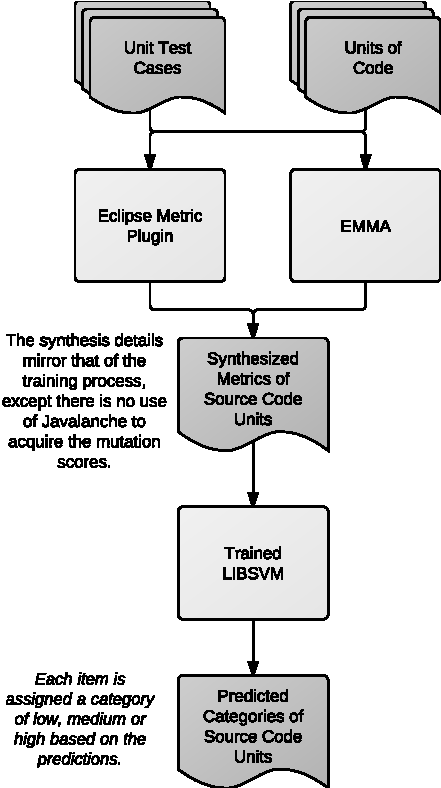
\includegraphics[width=7cm]{figures/process_prediction.pdf}
  \caption{Our prediction process for predicting mutation scores of source code units given a trained \gls{svm}.}
  \label{fig:process_prediction}
  \vspace{2mm}
  \hrule
\end{figure}

Once we have trained the \gls{svm}, we can then use it for prediction. We can predict the mutation score category of an unknown source code unit by first determining the source code and test suite metrics. The metrics (i.e., attributes) are passed into the \gls{svm} model which will then assign a category of \textit{low, medium, high} for the mutation score. As shown in Figure~\ref{fig:process_prediction} our prediction process is not too different from the training process, we now can exclude \emph{Javalanche} from the process~\footnote{We currently calculate the \emph{NOT} (i.e., number of tests) attribute using Javalanche, though ideally we can calculate this using \emph{EMMA}. This is a setback in our current implementation.}.


\section{Related Work}
\label{sec:approach_related_work}
Although prediction of mutation scores has not been previously researched, the related topic of using software metrics to locate faults in source code has been well researched. For example, Koru and Liu utilized static software measure along with defect data at the class level to predict bugs using machine learning~\cite{KL05}. Similarly, Gyimothy et al. used object-oriented metrics with logistic regression and machine learning techniques to identify faulty classes in open source software~\cite{GFS05}. Design level metrics were used with a linear prediction model to determine the estimated maintainability and error prone modules of large software systems~\cite{MKPS00}. Nagappan et al. used post-release defects of multiple versions along with source code complexity metrics to predict component failures~\cite{NBZ06}. Our work is unique in comparison to these previous works since we not only use source code metrics but we also use test suite metrics to enhance our predication capabilities. The aforementioned works on fault prediction do not use test suite metrics for their predictions, however they do, in some cases, utilize bug reports.

Wong et al. used statement coverage of test cases to localize faults using different heuristics~\cite{WDC10}. The aforementioned studies primarily utilized source code metrics, this study used only test suite metrics for fault localization. On a more related study, Anderson et al. used a neural network to prune a test suite preserved test suite effectiveness for domain based testing~\cite{AMM95}. Their approach uses attributes of test cases as input and an oracle that determined the severity of faults present in test cases. This study does not examine the \gls{sut}'s source code metrics, and focuses entirely on the test suite. They used test suite metrics such as the length of the test case and command/parameter frequency.

Nagappan et al. created the \emph{Software Testing and Reliability Early Warning (STREW) metric suite}, a test quality indicator~\cite{NWO+05, NWVO05}. Both source source code and test suite metrics are used in their calculation of test quality, which is the closest use of metrics to our own set.

Laura researched the relationship between test suite size, basic block coverage and test suite effectiveness~\cite{Ino12}. This study is related as Laura used EMMA to measure basic block coverage and Javalanche to measure test suite effectiveness, which is very similar to our approach. The research question between their study and ours are quite different. We are trying to predict the mutation score (i.e., the test suite effectiveness) of individual source code units. Laura's study attempts to understand whether basic block coverage and test suite size are effective in predicting test suite effectiveness. Laura determined that basic block coverage is a poor predictor of test suite effectiveness. 


\section{Summary}
\label{sec:approach_summary}
In this chapter we covered all aspects of our approach in terms of tools and the process used to collect and train our \gls{svm}. As we use a \gls{svm} as our prediction technique we require training data, thus we collected the mutation scores of each source code unit. We also collected the various metrics from the source code and test suite and synthesized all the acquire data to train our \gls{svm} to make prediction on existing and new data. We described each step of our process in Section~\ref{sec:approach_process}, and how we perform prediction in Section~\ref{sec:approach_prediction}. Finally in Section~\ref{sec:approach_related_work} we addressed related work to our approach on prediction of mutation scores using machine learning prediction techniques.
